\documentclass[aspectratio=169,11pt]{beamer}
\usetheme{default}
\usepackage[T1]{fontenc}
\usepackage{lmodern}
\usepackage{booktabs,tikz,xcolor,array}
\usetikzlibrary{positioning,arrows.meta}
\graphicspath{{figures/}{../../results/plots/}{../figures/}{../demo/}{../../logs/qgis_session/charts/}}

% ---------------------------------------------------------------- look (navy + orange, as in the team deck)
\definecolor{navy}{HTML}{1F3A5F}
\definecolor{accent}{HTML}{D9622B}
\definecolor{band}{HTML}{DCE3EC}
\definecolor{ink}{HTML}{1C1E22}
\definecolor{ink2}{HTML}{55595F}
\definecolor{okgreen}{HTML}{1B8A5A}
\usefonttheme{professionalfonts}
\setbeamertemplate{navigation symbols}{}
\setbeamercolor{normal text}{fg=ink}
\setbeamercolor{structure}{fg=navy}
\setbeamercolor{title}{fg=navy}
\setbeamercolor{subtitle}{fg=navy}
\setbeamercolor{alerted text}{fg=accent}
\setbeamercolor{frametitle}{bg=band,fg=navy}
\setbeamercolor{framesubtitle}{fg=navy}
\setbeamercolor{livebox}{bg=band,fg=ink}
\setbeamerfont{title}{size=\LARGE,series=\bfseries}
\setbeamerfont{frametitle}{size=\large,series=\bfseries}
\setbeamerfont{framesubtitle}{size=\footnotesize,series=\bfseries}
\makeatletter
\setbeamertemplate{frametitle}{\nointerlineskip
  \begin{beamercolorbox}[wd=\paperwidth,leftskip=1em,rightskip=1em,sep=0.45em]{frametitle}
  \usebeamerfont{frametitle}\insertframetitle
  \ifx\insertframesubtitle\@empty\else\\[-1pt]{\usebeamerfont{framesubtitle}\insertframesubtitle}\fi
  \end{beamercolorbox}\vspace{0.3em}}
\makeatother
\setbeamertemplate{footline}{\hfill{\scriptsize\color{ink2}\insertframenumber/\inserttotalframenumber}\hspace{1em}\vspace{0.5em}}
\setbeamertemplate{itemize items}[triangle]
\setbeamertemplate{enumerate items}[default]

\newcommand{\stat}[2]{\begin{tabular}[t]{@{}c@{}}{\LARGE\bfseries\color{accent}#1}\\[-1pt]{\scriptsize #2}\end{tabular}}
\newcommand{\stats}[2]{\begin{tabular}[t]{@{}c@{}}{\Large\bfseries\color{accent}#1}\\[-1pt]{\tiny #2}\end{tabular}}
\newcommand{\src}[1]{\par\vfill{\tiny\color{ink2}Source: #1}}
\newcommand{\live}[1]{\begin{beamercolorbox}[wd=\linewidth,sep=0.4em,rounded=true]{livebox}%
  \small\textbf{\color{accent}LIVE}\quad #1\end{beamercolorbox}}

\title{GeoGuessers}
\subtitle{Testing \& optimizing spatial calculation algorithms on a laptop}
\author{Swayam Goyal \and Siddharth Choudhary \and Yakkala Viswanadha Kartikeya}
\institute{Spatial Informatics \textbar{} Final project presentation}
\date{November 2026}

\begin{document}

\begin{frame}[plain]
\titlepage
\end{frame}

\newcommand{\half}[1]{{\small\bfseries\color{navy}#1}\par\vspace{-2pt}{\color{band}\rule{\linewidth}{1.2pt}}\par\vspace{1pt}}
% ================================================================ 1. motivation
\newcommand{\takeaway}[1]{\begin{beamercolorbox}[wd=\linewidth,sep=0.5em,rounded=true]{livebox}%
  \small\bfseries\color{navy}#1\end{beamercolorbox}}

\begin{frame}{The problem}
\framesubtitle{Where do standard terrain tools stop being practical on a laptop, and why?}
\begin{columns}[c]
\column{0.60\textwidth}
\centering
\stat{43\,GB}{1\,m DEM of our area}\hfill
\stat{16\,GB}{laptop RAM}\hfill
\stat{10.8\,B}{cells to process}
\vspace{14pt}
\begin{flushleft}
\small
\begin{enumerate}\setlength\itemsep{4pt}
  \item \textbf{Where is the real bottleneck?}
  \item \textbf{What does computing on demand from the pyramid cost and save?}
  \item \textbf{Can it keep up with continuous pan and zoom?}
\end{enumerate}
\end{flushleft}
\column{0.38\textwidth}
\centering
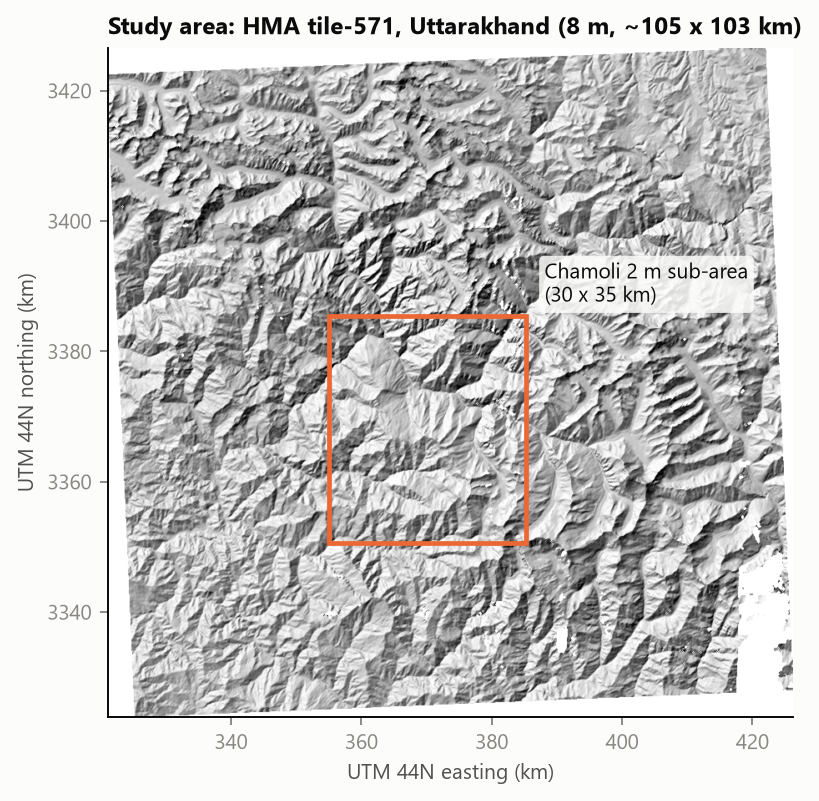
\includegraphics[width=\linewidth,height=0.66\textheight,keepaspectratio]{study_area.png}\\
{\tiny\color{ink2}Chamoli, Himalaya: 90\,m to 2\,m real, 1\,m synthetic}
\end{columns}
\end{frame}

\begin{frame}{What we changed, and why}
\framesubtitle{Each change answers one measured bottleneck}
\centering
\renewcommand{\arraystretch}{1.4}
\begin{tabular}{lcl}
\toprule
Baseline finding & & Our change \\
\midrule
Computing runs on one thread & $\to$ & Parallel compiled kernel (Numba) \\
Decompression and writing block computing & $\to$ & Reader threads + a writer thread \\
Three products need three passes & $\to$ & One fused kernel \\
Memory must stay flat & $\to$ & 2048$^2$ windows with a 1-cell halo \\
Still CPU-limited & $\to$ & GPU engine (CUDA) \\
{\color{accent}99.98\% of cells are off-screen} & $\to$ & {\color{accent}On demand from the pyramid} \\
\bottomrule
\end{tabular}
\end{frame}

% ================================================================ 2. baseline
\begin{frame}{Baseline: gdaldem doesn't break, it slows down}
\begin{columns}[c]
\column{0.58\textwidth}
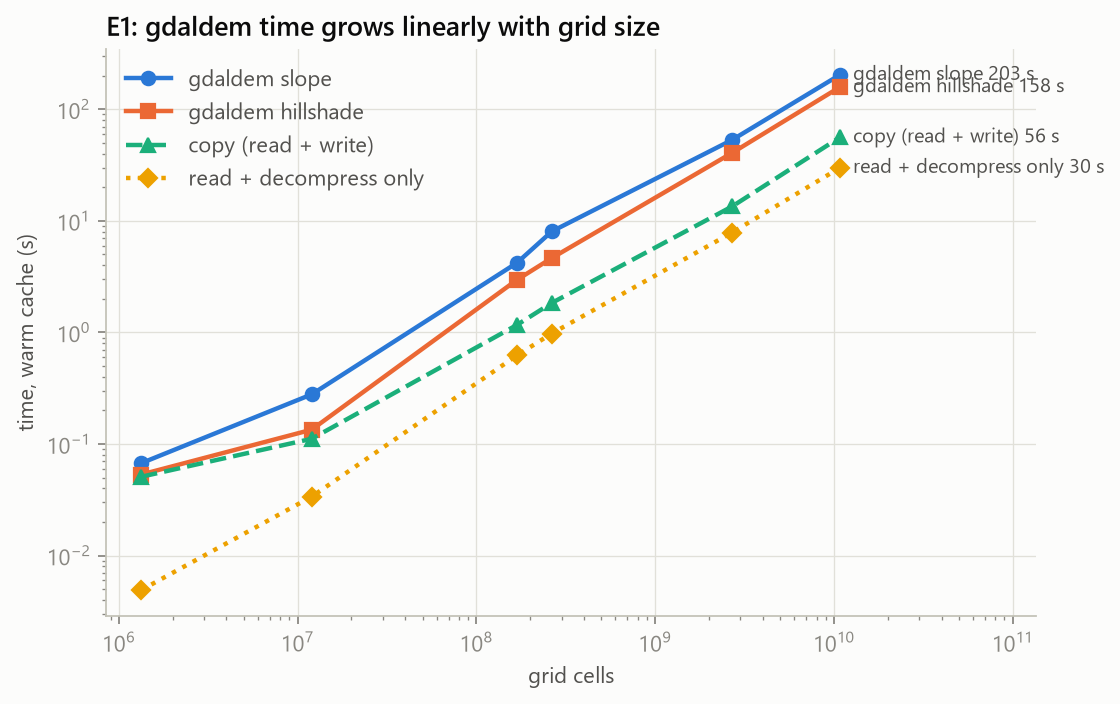
\includegraphics[width=\linewidth]{e1_scaling.png}
\column{0.40\textwidth}
\centering
\stat{208\,s}{slope at 1\,m}\hfill\stat{0.87\,GB}{RAM, at any size}\\[14pt]
\stat{73\%}{time spent computing}\hfill\stat{1 / 22}{threads used}\\[16pt]
\takeaway{Not the disk, not memory: one thread computing.}
\end{columns}
\end{frame}

\begin{frame}{Baseline: for display, the pyramid is everything}
\begin{columns}[c]
\column{0.58\textwidth}
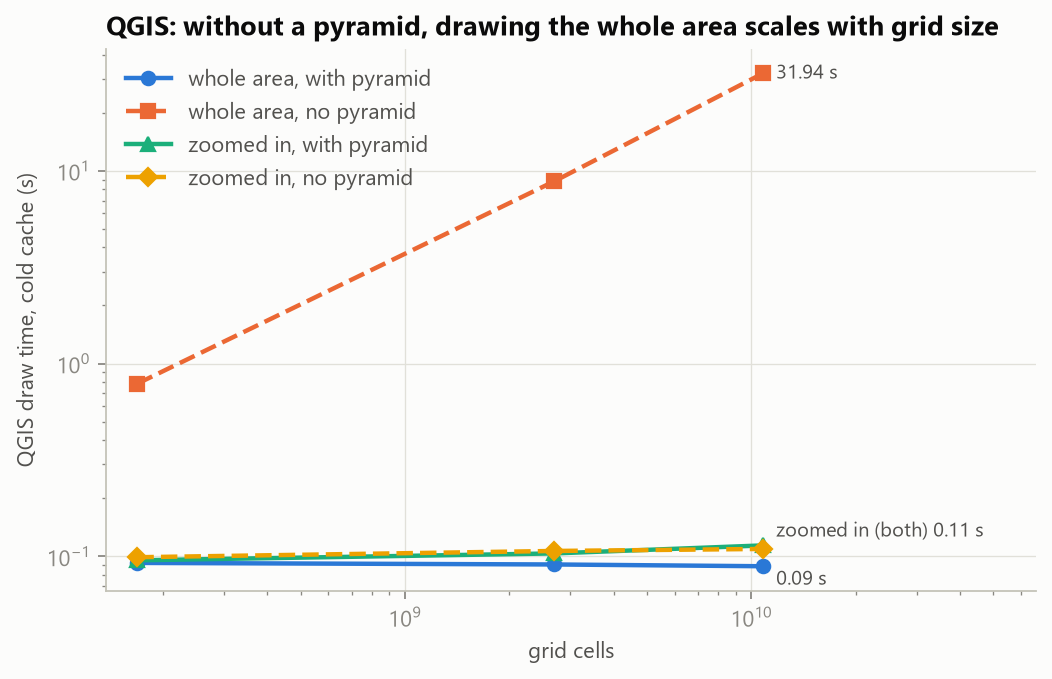
\includegraphics[width=\linewidth]{e1q_render.png}
\column{0.40\textwidth}
\centering
\stat{31.9\,s}{QGIS redraw, no pyramid}\hfill\stat{0.09\,s}{with a pyramid}\\[14pt]
\stat{2.9$\times$}{smaller with ZSTD (our COG format)}\\[16pt]
\takeaway{A screen shows $\sim$2\,M pixels. Why compute 10.8\,B cells?}
\end{columns}
\end{frame}

% ================================================================ 3. engines
\begin{frame}{Our CPU engine: parallel, flat memory, exact}
\begin{columns}[c]
\column{0.58\textwidth}
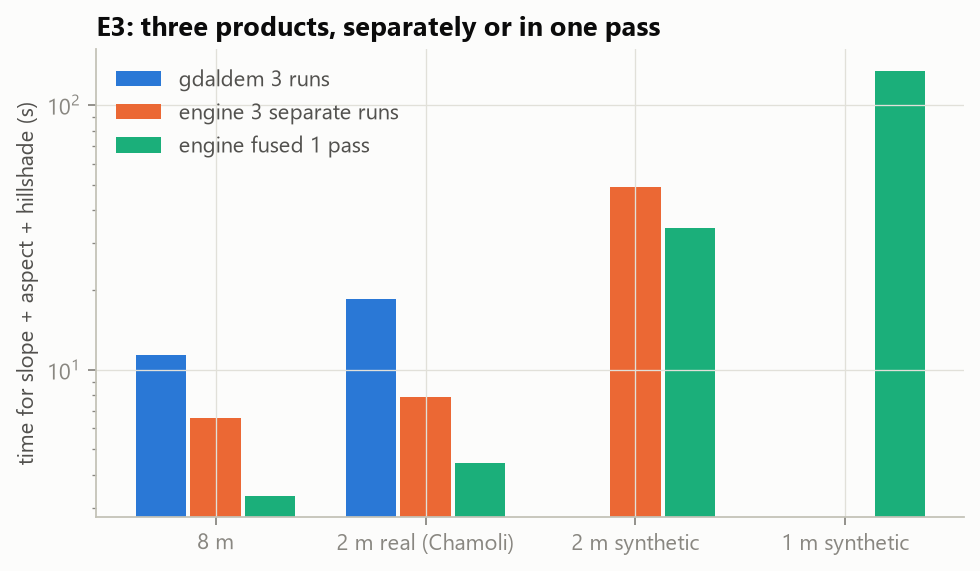
\includegraphics[width=\linewidth]{e3_products.png}
\column{0.40\textwidth}
\centering
\stat{3.5$\times$}{faster (208\,s $\to$ 60\,s)}\hfill\stat{1.4\,GB}{RAM, at any size}\\[14pt]
\makebox[0.5\linewidth]{\stat{3.4--4.2$\times$}{3 products, 1 pass}}\makebox[0.5\linewidth]{\stat{0}{cells differ (gdaldem)}}\\[16pt]
\takeaway{Readers $\to$ parallel kernel $\to$ writer, in bounded windows.}
\end{columns}
\end{frame}

\begin{frame}{GPU engine: fast kernel, small overall gain}
\begin{columns}[c]
\column{0.58\textwidth}
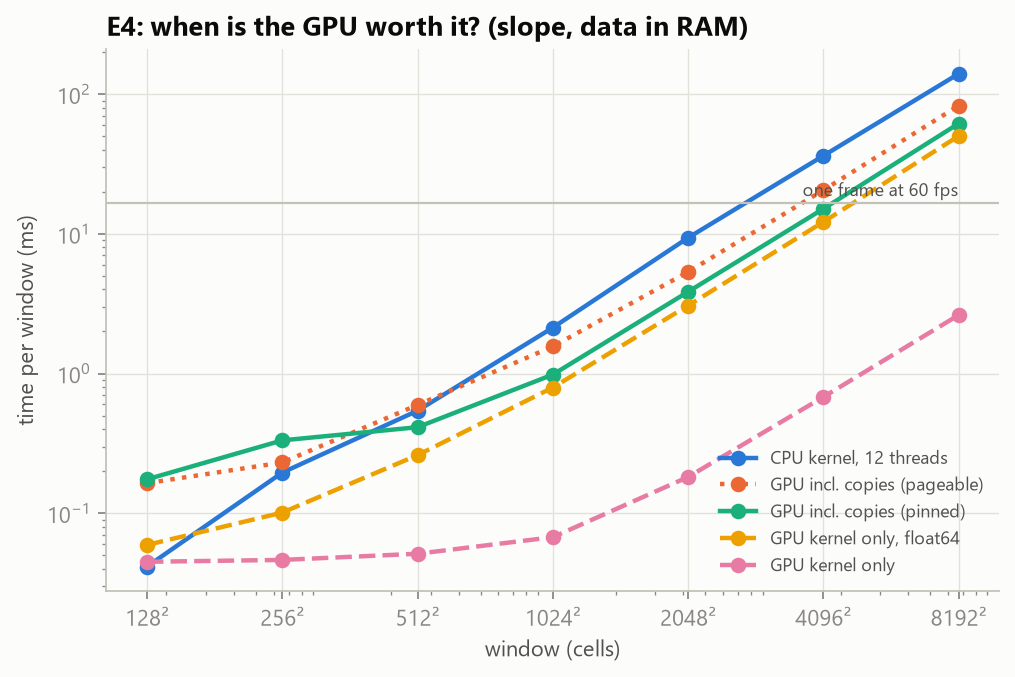
\includegraphics[width=\linewidth]{e4_crossover.png}
\column{0.40\textwidth}
\centering
\stat{50$\times$}{kernel vs CPU}\hfill\stat{1.4$\times$}{whole run vs CPU}\\[14pt]
\stat{95\%}{of GPU time is copying}\hfill\stat{4.75$\times$}{vs gdaldem (43.8\,s)}\\[16pt]
\takeaway{The GPU computes fast but waits for data.}
\end{columns}
\end{frame}

\begin{frame}{The bottleneck moves, so compute only what is seen}
\begin{columns}[c]
\column{0.58\textwidth}
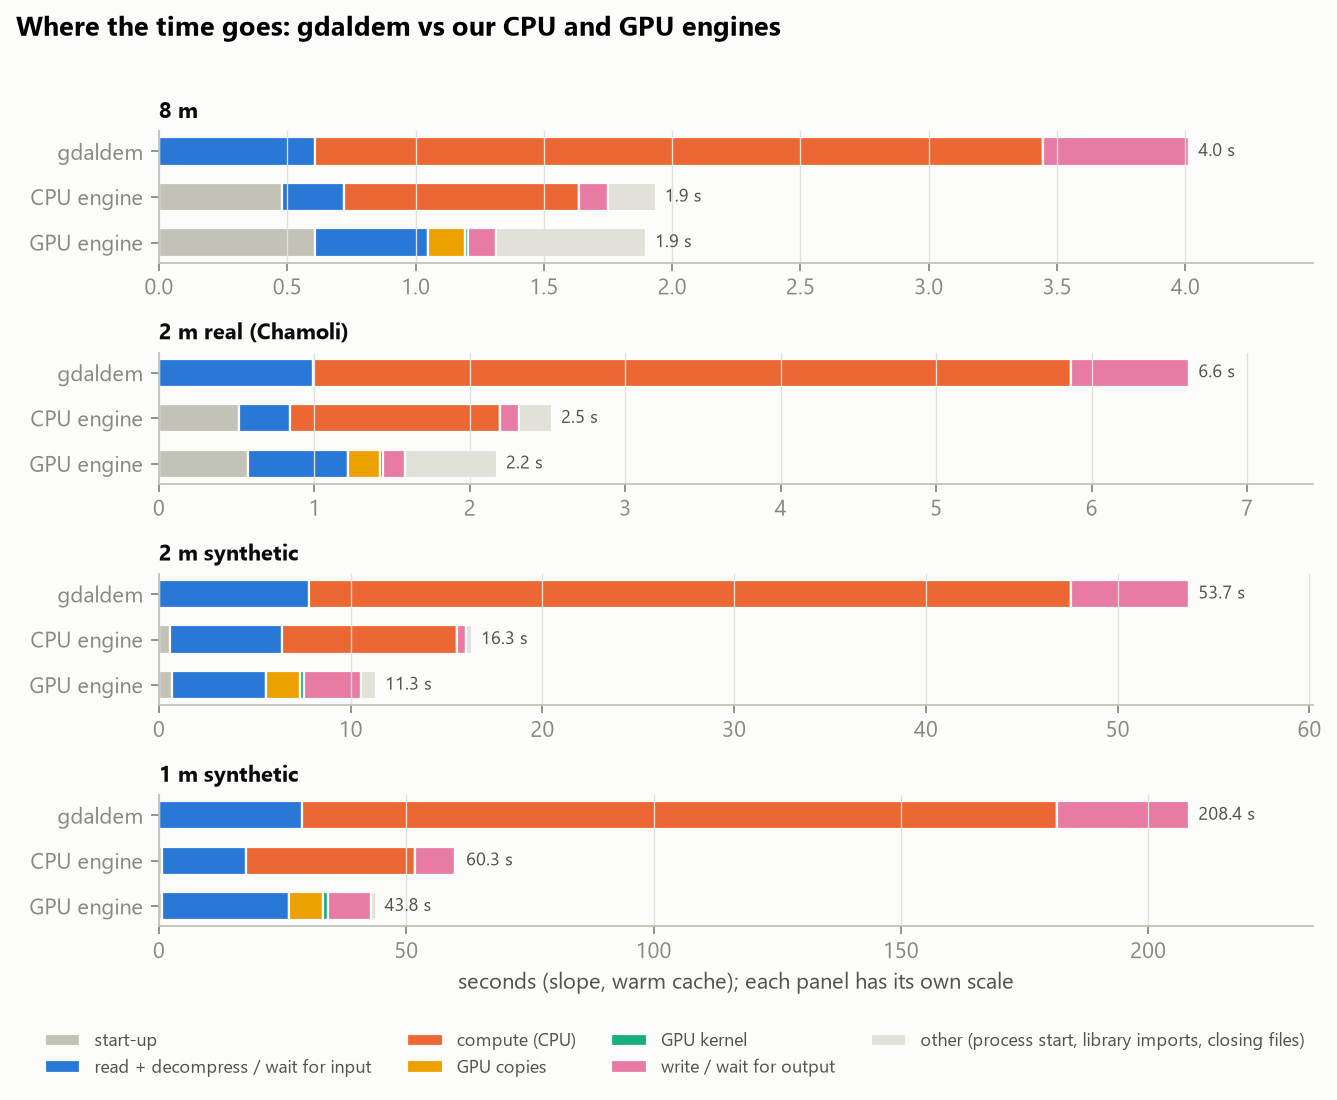
\includegraphics[width=\linewidth,height=0.80\textheight,keepaspectratio]{e4_stages.png}
\column{0.40\textwidth}
\centering
{\large\bfseries\color{navy} computation $\to$ decompression $\to$ writing}\\[14pt]
\stat{33\,s}{computing at 1\,m}\hfill\stat{65\,s}{writing at 1\,m}\\[16pt]
\takeaway{Faster kernels no longer help. Read and write less: derive on demand from the pyramid level that fits
the screen.}
\end{columns}
\end{frame}

% ================================================================ 4. on demand
\begin{frame}{On-demand derivatives from the pyramid}
\framesubtitle{Compute only what is viewed, at the resolution that fits the screen}
\begin{columns}[c]
\column{0.55\textwidth}
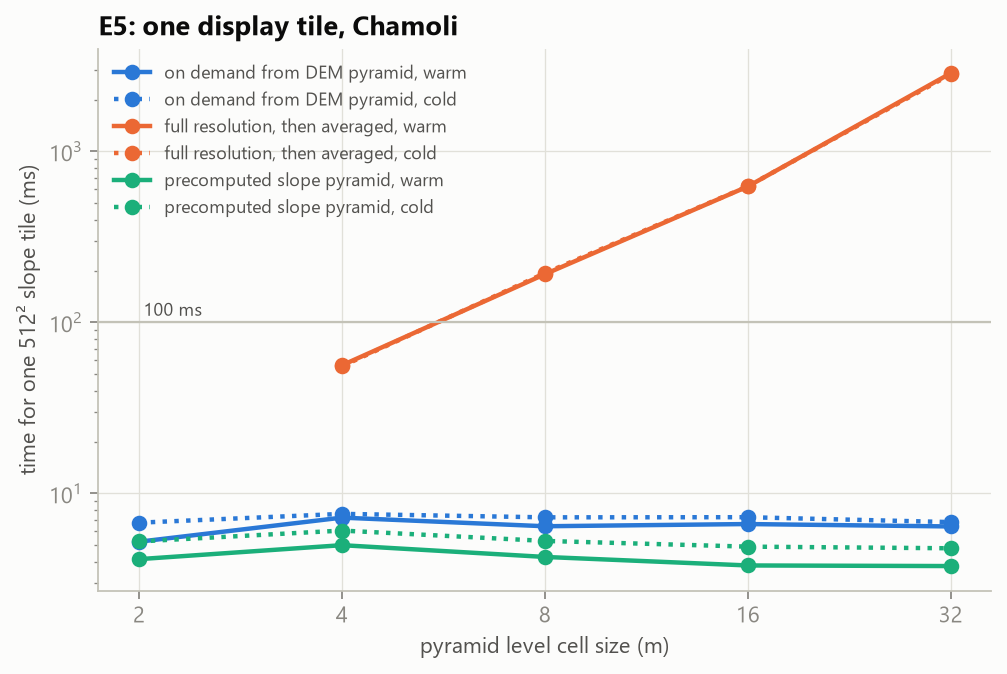
\includegraphics[width=\linewidth]{e5_tile_time.png}
\column{0.43\textwidth}
\centering
\stat{5--8\,ms}{per 512$^2$ tile, any zoom}\hfill\stat{447$\times$}{vs exact at 32\,m}\\[6pt]
\stat{0\,GB}{precomputed storage}\\[6pt]
\small
\begin{itemize}
  \item Read one 512$\times$512 window (+1 halo) from the COG level that fits the screen
  \item Exact tiles: 56\,ms (4\,m) to 2.9\,s (32\,m)
  \item New sun angle or product: nothing to rebuild (a slope pyramid costs 1.0\,GB per product)
\end{itemize}
\end{columns}
\src{E5, final report}
\end{frame}

\begin{frame}{Accuracy vs speed: the pyramid trade-off}
\framesubtitle{The price of speed is slope that is too low; aspect survives well}
\begin{columns}[c]
\column{0.48\textwidth}
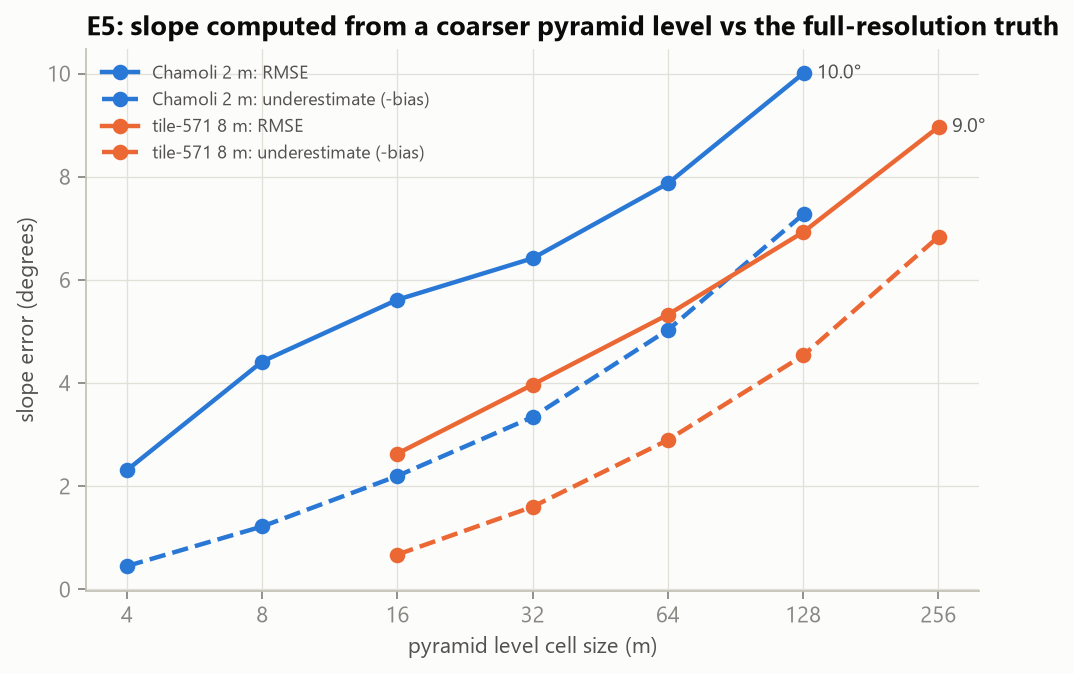
\includegraphics[width=\linewidth]{e5_error_by_level.png}
\column{0.50\textwidth}
\centering
\stats{2.3$^\circ$}{RMSE, 1 level up}\hfill\stats{6.4$^\circ$}{RMSE, 4 levels up}\hfill\stats{2--8$^\circ$}{aspect median error}\\[6pt]
\small
\begin{itemize}
  \item Rule of thumb: $\approx$2.5$^\circ$ one level up, +1.5$^\circ$ per further level; almost all
  \textbf{underestimates}
  \item Steep ground loses most: cells $\geq$45$^\circ$ drop from 29\% to 22\% at 32\,m
  \item A pyramid level beats an independent DEM of the same cell size
  \item \textbf{Auto} mode for display; \textbf{Exact} mode for thresholds and hazard maps
\end{itemize}
\end{columns}
\src{E5 against the Chamoli 2\,m truth, final report}
\end{frame}

% ================================================================ 5. system
\begin{frame}{End-to-end system}
\centering
\resizebox{0.95\linewidth}{!}{%
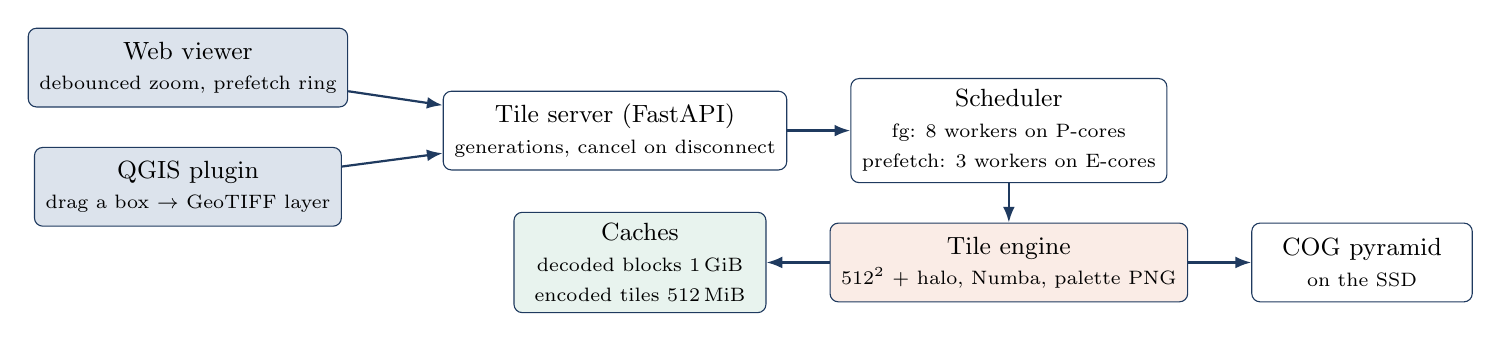
\begin{tikzpicture}[node distance=5mm and 8mm, box/.style={draw=navy, rounded corners=3pt, align=center,
  font=\small, minimum height=10mm, inner sep=4pt, fill=white}, arr/.style={-{Latex[length=2mm]}, navy, thick}]
  \node[box, fill=band] (web) {Web viewer\\{\scriptsize debounced zoom, prefetch ring}};
  \node[box, fill=band, below=of web] (qgis) {QGIS plugin\\{\scriptsize drag a box $\to$ GeoTIFF layer}};
  \node[box, right=12mm of web, yshift=-8mm, minimum width=32mm] (srv) {Tile server (FastAPI)\\{\scriptsize generations,
    cancel on disconnect}};
  \node[box, right=of srv, minimum width=36mm] (sch) {Scheduler\\{\scriptsize fg: 8 workers on P-cores}\\{\scriptsize
    prefetch: 3 workers on E-cores}};
  \node[box, below=of sch, minimum width=36mm, fill=accent!12] (eng) {Tile engine\\{\scriptsize 512$^2$ + halo, Numba,
    palette PNG}};
  \node[box, left=of eng, minimum width=32mm, fill=okgreen!10] (cache) {Caches\\{\scriptsize decoded blocks 1\,GiB}\\{\scriptsize
    encoded tiles 512\,MiB}};
  \node[box, right=of eng, minimum width=28mm] (cog) {COG pyramid\\{\scriptsize on the SSD}};
  \draw[arr] (web) -- (srv); \draw[arr] (qgis) -- (srv); \draw[arr] (srv) -- (sch); \draw[arr] (sch) -- (eng);
  \draw[arr] (eng) -- (cache); \draw[arr] (eng) -- (cog);
\end{tikzpicture}}
\vspace{10pt}
\footnotesize
\renewcommand{\arraystretch}{1.3}
\begin{tabular}{>{\raggedleft\arraybackslash\color{navy}\bfseries}l l}
Block cache & Decoded blocks shared by all tiles; without it 6$\times$ more decodes, p95 +40\% \\
Scheduler & Visible tiles first; a visible request promotes a queued prefetch \\
Cancellation & New generation per pan or zoom; aborted requests dropped in a median 37\,ms \\
\end{tabular}
\src{\texttt{docs/PHASE5\_RESULTS.md}, final report}
\end{frame}

\begin{frame}{Viewer: the debounce cuts server work 3.3$\times$}
\begin{columns}[c]
\column{0.60\textwidth}
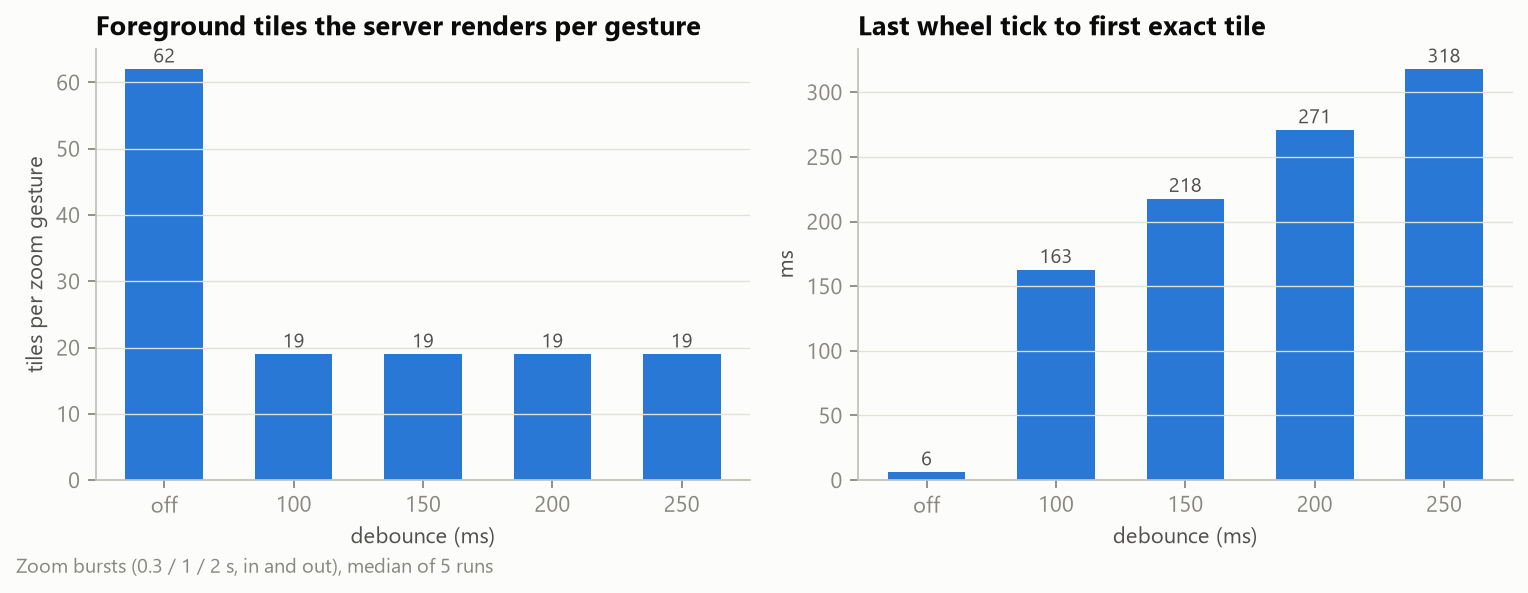
\includegraphics[width=\linewidth]{e6_debounce.png}
\column{0.38\textwidth}
\centering
\stat{62 $\to$ 19}{server tiles per zoom}\hfill\stat{63--71\,ms}{first exact tile after commit}\\[6pt]
\small
\begin{itemize}
  \item Each wheel tick moves the camera at once; cached tiles stand in
  \item One commit \textbf{150\,ms} after the last tick
  \item Notched wheel: 100\,ms is as bad as none (36 tiles), 150\,ms coalesces (15)
\end{itemize}
\end{columns}
\src{E6, final report}
\end{frame}

\begin{frame}{Viewer: prefetch makes panning seamless}
\begin{columns}[c]
\column{0.55\textwidth}
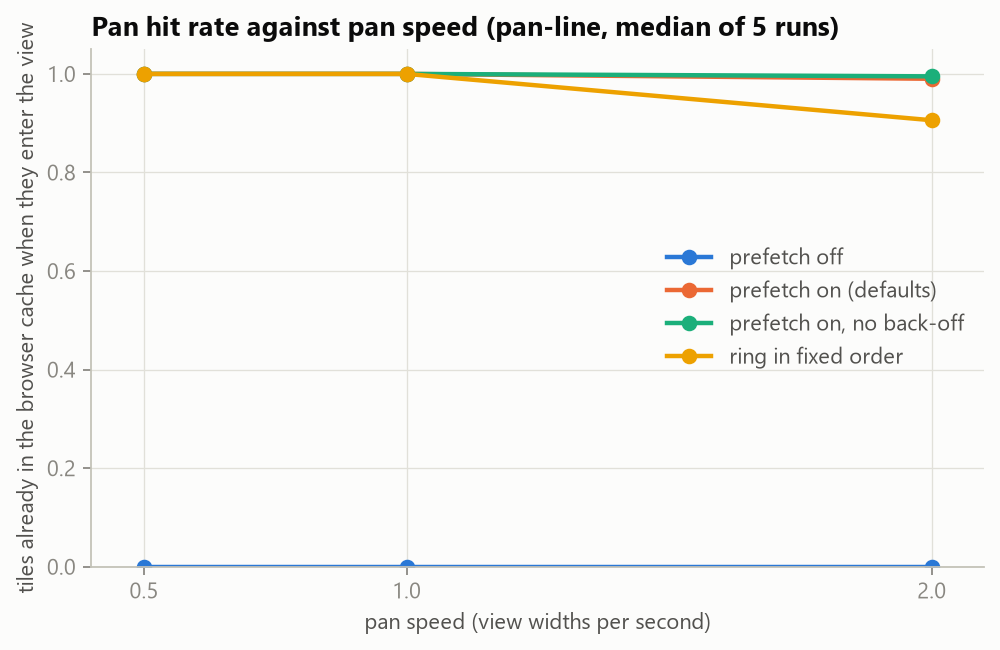
\includegraphics[width=\linewidth]{e6_hit_vs_speed.png}
\column{0.43\textwidth}
\centering
\stat{98--100\%}{tiles already there when panned in}\hfill\stat{90 vs 95\,ms}{server p95, prefetch on / off}\\[6pt]
\small
\begin{itemize}
  \item 8 neighbouring views at low priority, direction of travel first
  \item Without prefetch: 0\% on a straight pan
  \item \textbf{Does not slow visible tiles}: all 122{,}215 prefetch jobs ran on E-cores
  \item Server peak 982\,MiB; full view 76--158\,ms after a zoom
\end{itemize}
\end{columns}
\src{E6, final report}
\end{frame}

\begin{frame}{Live demo: the web viewer}
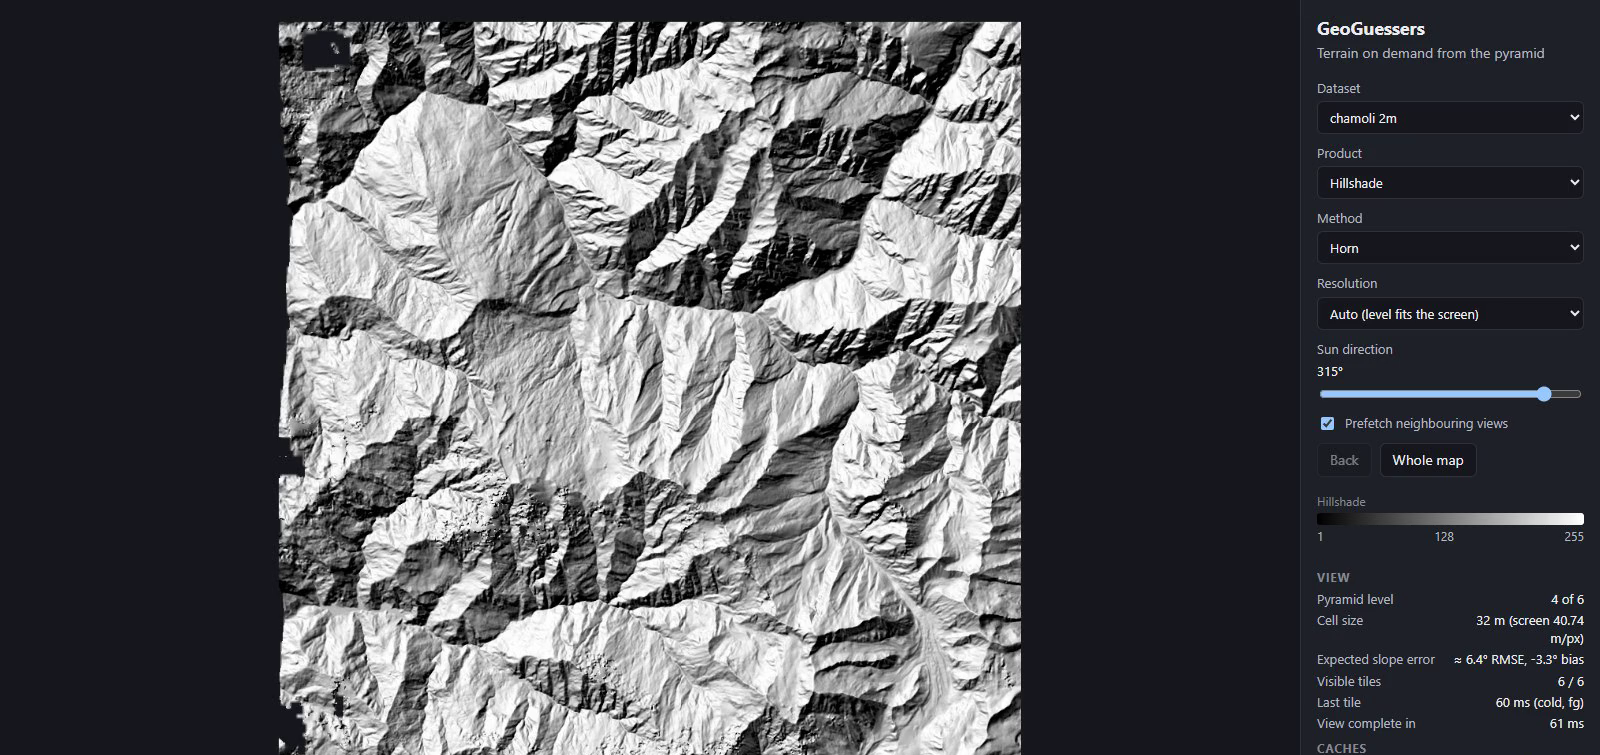
\includegraphics[width=0.325\linewidth]{viewer_2.png}\hfill
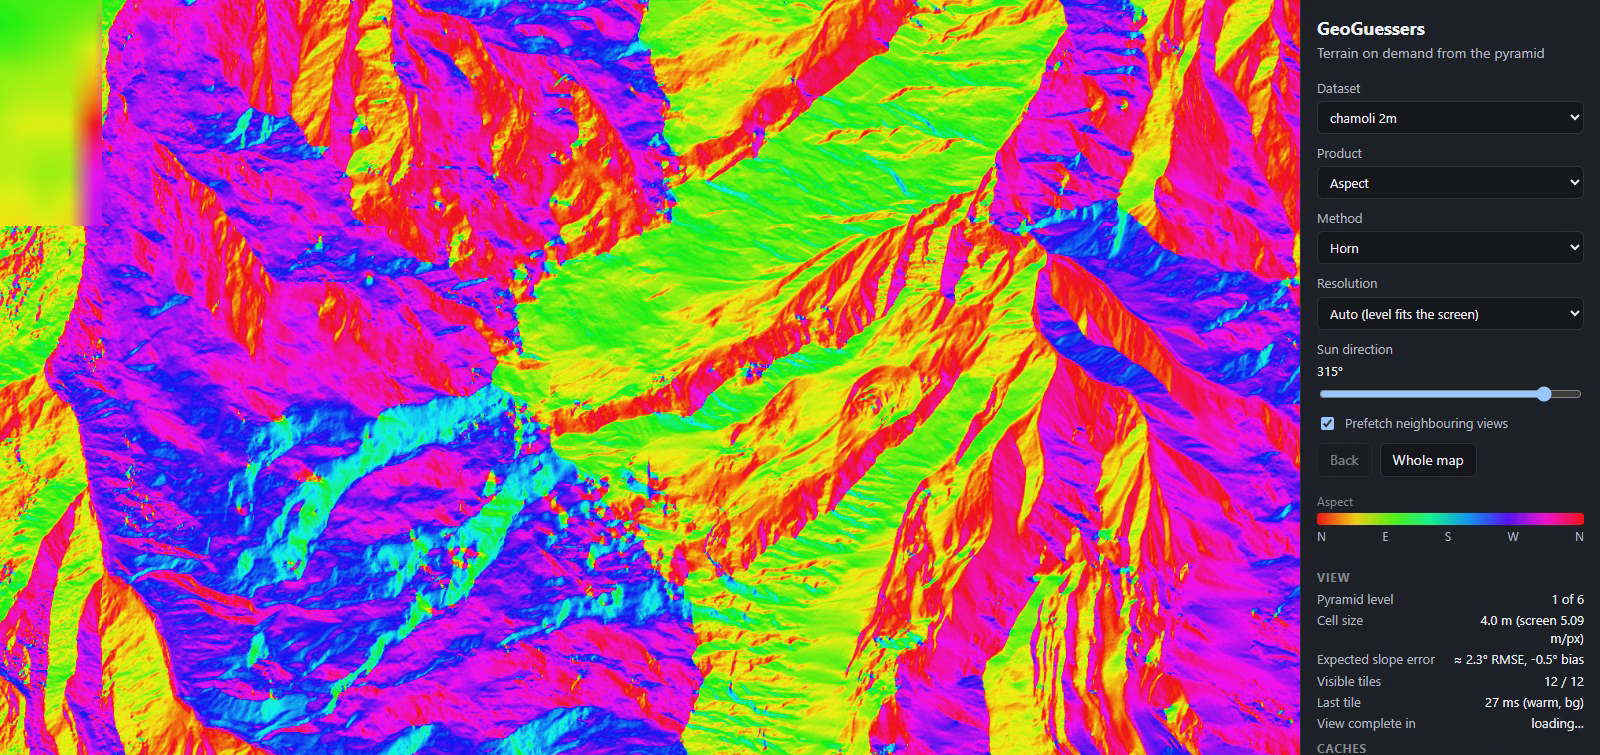
\includegraphics[width=0.325\linewidth]{viewer_17.png}\hfill
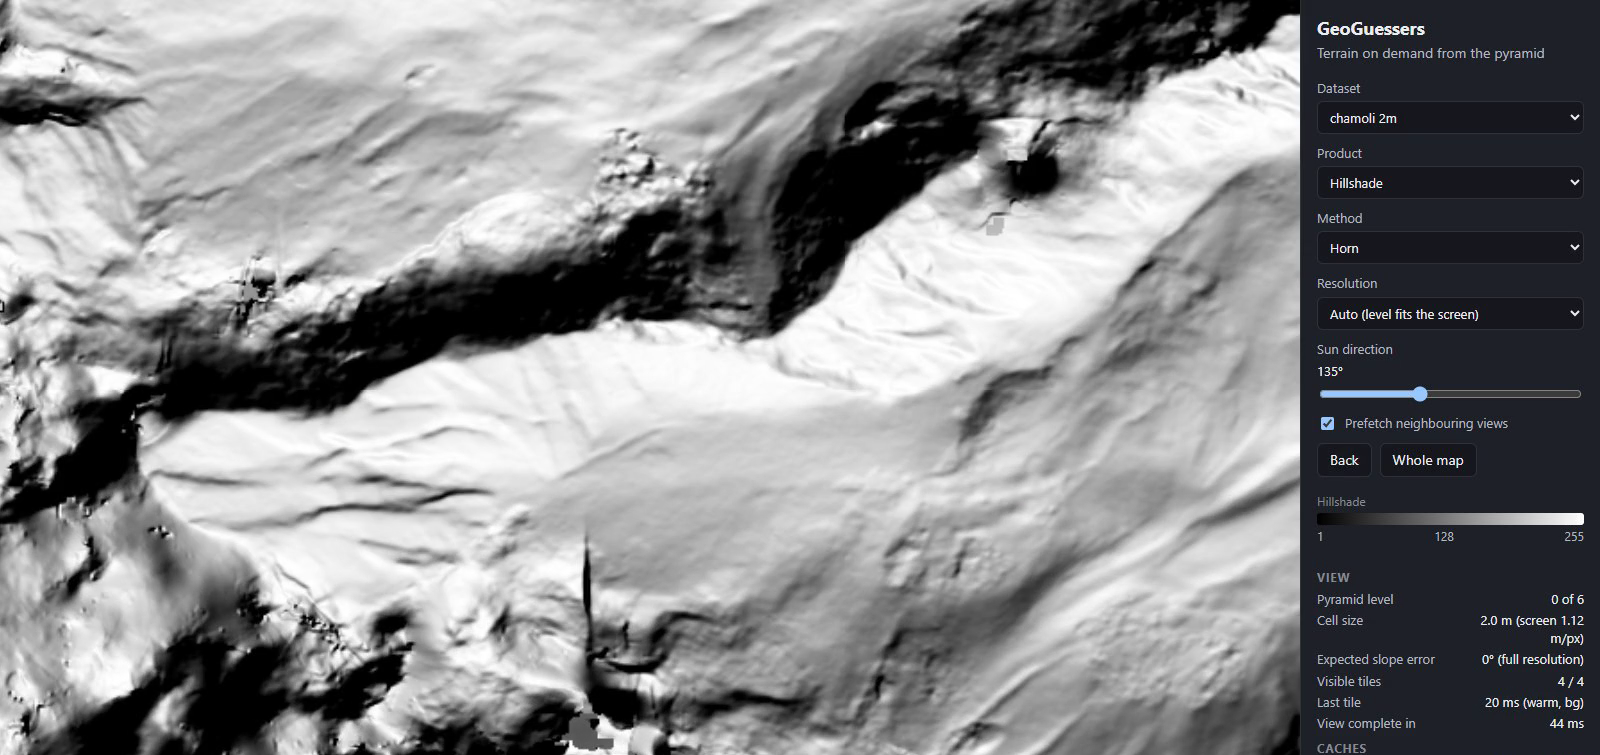
\includegraphics[width=0.325\linewidth]{viewer_31.png}\\[-2pt]
{\tiny\color{ink2}\makebox[0.325\linewidth]{Whole map, coarse level}\hfill\makebox[0.325\linewidth]{Aspect, on demand}\hfill
\makebox[0.325\linewidth]{Full resolution (2\,m cells)}}
\vspace{6pt}
\live{\texttt{python -m server}\quad then open\quad \texttt{http://127.0.0.1:8765/viewer/}}
\vspace{4pt}
\small
\begin{columns}[T]
\column{0.5\textwidth}
\begin{enumerate}
  \item Wheel zoom: preview tiles, then one commit
  \item Pan: prefetched tiles already there
  \item Switch product: slope, aspect, TPI
\end{enumerate}
\column{0.5\textwidth}
\begin{enumerate}\setcounter{enumi}{3}
  \item Drag the sun direction (hillshade)
  \item Shift + drag a box down to 2\,m cells
  \item Status panel: level, cell size, expected error
\end{enumerate}
\end{columns}
\end{frame}

\begin{frame}{QGIS plugin: native interactive integration}
\begin{columns}[c]
\column{0.50\textwidth}
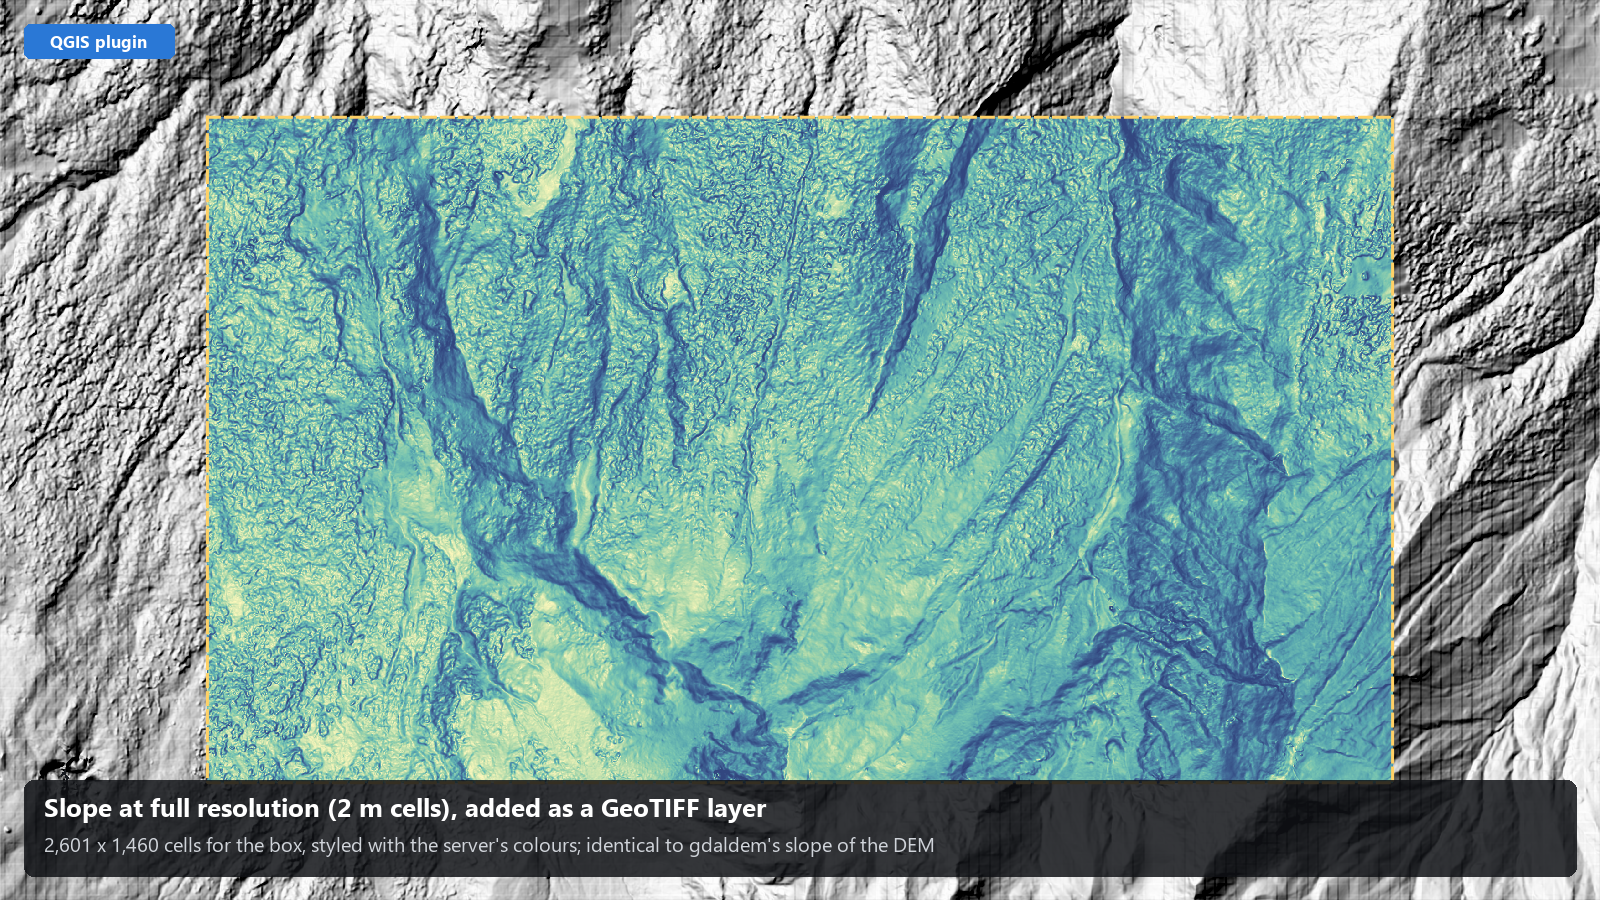
\includegraphics[width=\linewidth]{qgis_q3.png}\\
{\tiny\color{ink2}A 2\,m slope box drawn in QGIS, served by the same tile server}
\column{0.48\textwidth}
\centering
\stats{10--225\,ms}{per box (2.85\,B-cell DEM)}\hfill\stats{43 / 44}{boxes, 7 products}\hfill\stats{0 diff}{vs gdaldem}\\[6pt]
\small
\begin{itemize}
  \item Drag a box $\to$ styled GeoTIFF layer, computed in the background
  \item Level follows the box on screen: 128\,m $\to$ 2\,m as boxes shrink
  \item Full-resolution box identical to gdaldem (1.22\,M cells, max difference 0)
  \item A 400\,M-cell box is refused in 1\,ms (limit 64\,M cells)
\end{itemize}
\vspace{2pt}
\live{QGIS $\to$ GeoGuessers terrain $\to$ Draw a box}
\end{columns}
\src{\texttt{logs/qgis\_session/experiment\_report.md} (runs 3, 5); final report}
\end{frame}

% ================================================================ 6. validation
\begin{frame}{Validation: 2.85 billion cells (Swiss Alps lidar)}
\framesubtitle{11$\times$ the Chamoli dataset, on a second laptop (Ryzen 7 7840HS, Linux, QGIS 4)}
\begin{columns}[T]
\column{0.44\textwidth}
\centering
\stats{6.9--15\,ms}{median tile, Auto mode}\quad\stats{0.01--0.02}{server cores (median)}\quad\stats{0\%}{GPU use}
\column{0.54\textwidth}
\footnotesize
\begin{itemize}
  \item swissALTI3D 2\,m: 60{,}000 $\times$ 47{,}500 cells, 5.6\,GB COG; 7 sessions (viewer, QGIS, both)
  \item Decompression is 52--55\% of a tile read from disk: \textbf{decoding, not computing}, is the cost
  \item CPU time: QGIS 62\%, tile server 22\%
\end{itemize}
\end{columns}
\vspace{2pt}
\centering
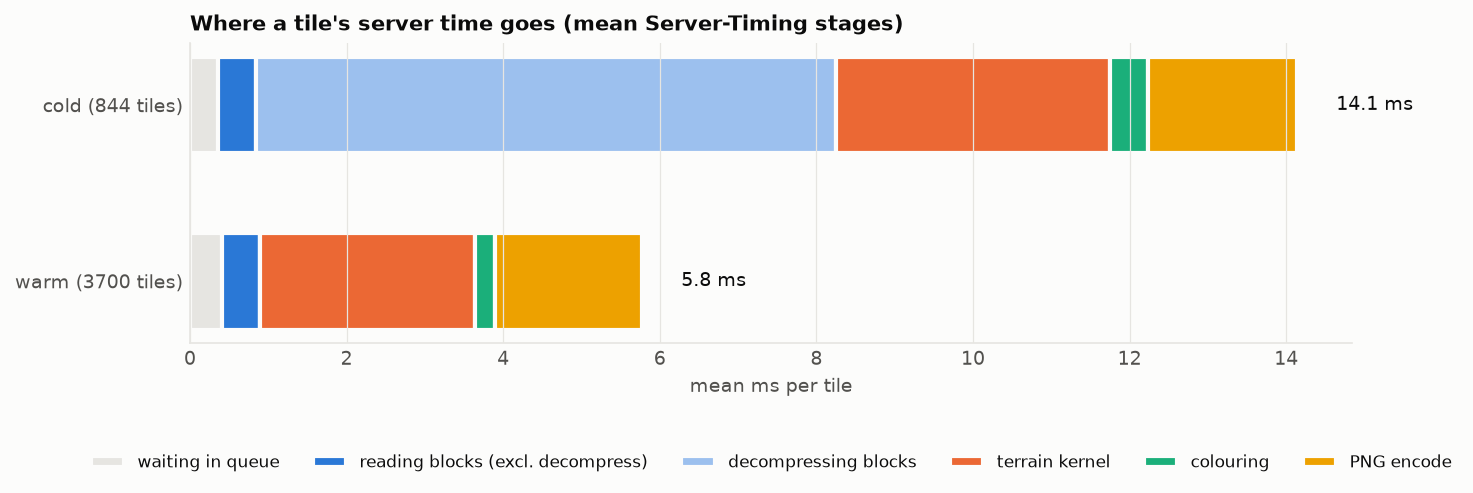
\includegraphics[width=0.74\linewidth]{run1_webview/tile_stages.png}\par
{\tiny\color{ink2}Where a tile's server time goes (run 1: 844 tiles read from disk, 3{,}700 with blocks already decoded)\par}
\src{\texttt{logs/qgis\_session/experiment\_report.md}; data \textcopyright{} swisstopo}
\end{frame}

\begin{frame}{Validation: where it breaks, Exact mode at this scale}
\centering
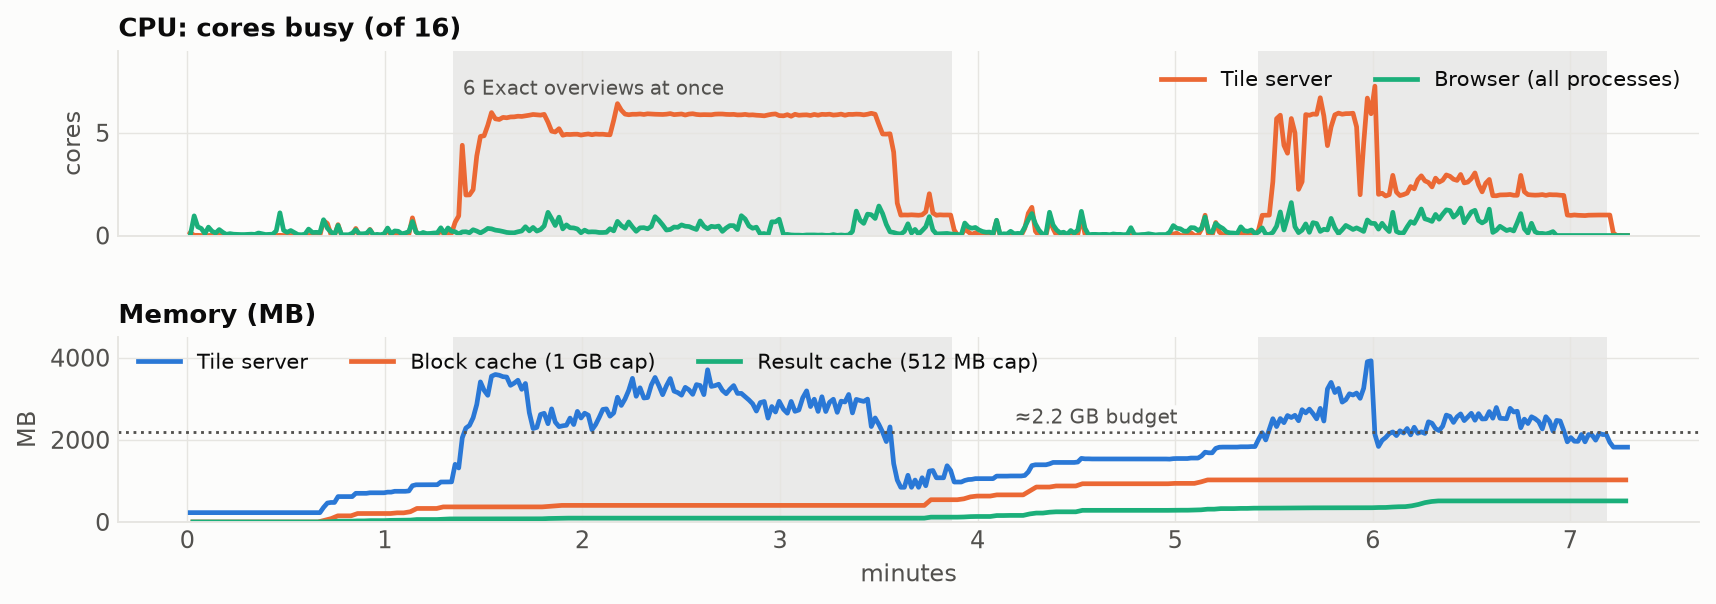
\includegraphics[width=0.84\linewidth]{swiss_run4_cpu_mem.png}\par
{\tiny\color{ink2}Run 4 (7.3\,min). Grey: Exact work running. Top: cores busy (tile server, browser); bottom: memory (MB)\par}
\vspace{2pt}
\footnotesize
\begin{columns}[T]
\column{0.49\textwidth}
\begin{itemize}
  \item \textbf{Auto mode stays at budget:} 1.9--2.3\,GB (full caches); $\sim$3\,GB may stay after Exact
  \item \textbf{Exact whole-map overview:} 47--129\,s on one core; server memory 2.9--4.9\,GB
\end{itemize}
\column{0.49\textwidth}
\begin{itemize}
  \item \textbf{Not cancelled:} each sun-direction change started a new overview; all 8 ran to completion
  \item \textbf{Fix:} build the overview from its own level, or cancel superseded overviews
\end{itemize}
\end{columns}
\src{\texttt{logs/qgis\_session/experiment\_report.md}, findings 1--3}
\end{frame}

% ================================================================ 7. wrap-up
\begin{frame}{Performance summary}
\centering
\small
\renewcommand{\arraystretch}{1.2}
\resizebox{\linewidth}{!}{%
\begin{tabular}{lrrrr}
\toprule
& \textbf{gdaldem} & \textbf{CPU engine} & \textbf{GPU engine} & \textbf{On demand (viewer)} \\
\midrule
Slope, 1\,m (10.8\,B cells) & 208\,s & 60\,s & 44\,s & \textbf{5--8\,ms per tile} \\
Speed-up & 1$\times$ & 3.5$\times$ & 4.75$\times$ & \textbf{8--450$\times$ vs exact tile} \\
Threads used & 1 of 22 & 12 P-core & CPU + GPU & \textbf{0.01--0.02 cores (median)} \\
Peak memory & 0.87\,GB & 1.4\,GB & $\leq$2.0\,GiB on GPU & \textbf{0.98--2.3\,GB} \\
Full-view redraw & 31.9\,s (QGIS, no pyramid) & -- & -- & \textbf{76--158\,ms after zoom} \\
Box in QGIS & -- & -- & -- & \textbf{10--225\,ms} (4.4\,s near the 64\,M-cell limit) \\
\bottomrule
\end{tabular}}
\vspace{6pt}
\begin{flushleft}\scriptsize\color{ink2}
Engines: whole-grid processing (E1, E3, E4). Viewer: E5 tiles, E6 (Chamoli, peak 982\,MiB) and the Swiss runs (2.85\,B
cells, up to 2.3\,GB with full caches; Exact overviews excluded, after which up to $\sim$3\,GB may be kept).
\end{flushleft}
\end{frame}

\begin{frame}{Conclusion}
\begin{enumerate}
  \setlength\itemsep{5pt}
  \item \textbf{Standard tools slow down, they don't fail.} gdaldem streams 43\,GB in 0.87\,GB but uses one thread.
  \item \textbf{Profile before assuming GPU.} Copies are 95\% of GPU time; the bottleneck moves from computing to
  decompressing and writing.
  \item \textbf{Never compute what cannot be seen.} On demand from the pyramid: 5--8\,ms per tile at any zoom,
  8--450$\times$ less than exact, 0\,GB storage.
  \item \textbf{Quantify the accuracy cost.} $\approx$2.5$^\circ$ slope RMSE one level up, +1.5$^\circ$ per further level;
  aspect within one compass sector.
  \item \textbf{Deliver it to the user.} Debounced, prefetching viewer and a QGIS plugin; holds at 2.85\,B cells.
\end{enumerate}
\end{frame}

\begin{frame}{Limitations and future work}
\begin{columns}[T]
\column{0.5\textwidth}
\textbf{Limitations}
\small
\begin{itemize}
  \item One study region of steep terrain (larger slope errors than flat land)
  \item Synthetic 2\,m / 1\,m grids for timing only
  \item E6: one client, short scripted traces; Swiss runs hand-driven
  \item Exact overviews: slow, uncancelled, over the memory budget
  \item Coarse-level slope bias not corrected
\end{itemize}
\column{0.5\textwidth}
\textbf{Future work}
\small
\begin{itemize}
  \item Cancel or cache Exact overviews
  \item Per-level slope bias correction
  \item Viewshed and terrain distance (G3)
  \item GPU tile path for bulk exports
  \item Decompress on the GPU to cut copies (est.\ up to 1.4$\times$)
  \item Several clients; cloud-hosted COGs
\end{itemize}
\end{columns}
\vfill
\centering\small Code, data manifests, results and reports: \url{https://github.com/Swayamgoyal/Geoguessers}
\end{frame}

\begin{frame}[plain]
\vfill\centering
{\Huge\bfseries\color{navy} Thank you}\\[10pt]
{\Large\color{accent} Questions?}\\[16pt]
{\small Team GeoGuessers \;\textperiodcentered\; Codebase and benchmarking harness available}
\vfill
\end{frame}

\end{document}
